\documentclass[conference]{IEEEtran}
\IEEEoverridecommandlockouts
\usepackage{cite}
\usepackage{amsmath,amssymb,amsfonts}
\usepackage{graphicx}
\usepackage{booktabs}
\usepackage{multirow}
\usepackage{xcolor}
\usepackage{tikz}
\usetikzlibrary{positioning,arrows.meta,fit,backgrounds}
\usepackage[hidelinks]{hyperref}

% ---------------------------------------------------------------------------
% Every red [TBD ...] marker is a number that has NOT been measured yet.
% Do not submit while any remain. PLACEHOLDERS.md lists the command that fills each one.
% ---------------------------------------------------------------------------
\newcommand{\TBD}[1]{\textcolor{red}{\textbf{[TBD: #1]}}}
\newcommand{\INR}{Rs.\,}
\newcommand{\tbd}{\textcolor{red}{\textbf{TBD}}}

\begin{document}

\title{SAHARA: Safety-Asymmetric, Privacy-Preserving On-Device Sound Awareness for Deaf and Hard-of-Hearing Users in Indian Homes}

\author{
\IEEEauthorblockN{Raj Singh, Prachi Teotia, Advika \TBD{surname}, Mahi \TBD{surname}, and \TBD{guide name}}
\IEEEauthorblockA{\textit{\TBD{Department}}, Mukesh Patel School of Technology Management and Engineering\\
SVKM's NMIMS, Mumbai, India\\
\TBD{corresponding e-mail}}
}

\maketitle

\begin{abstract}
Deaf and hard-of-hearing (DHH) people miss safety-critical sounds such as smoke alarms, sirens and breaking glass, yet most sound-recognition aids treat every class alike, send audio to the cloud, or are evaluated only on Western datasets. We present SAHARA, a fully on-device sound-awareness system that runs a frozen YAMNet encoder and a 296k-parameter classifier head inside an Android foreground service and relays alerts to a sub-\INR1000 ESP32 haptic wristband. SAHARA's central idea is \emph{safety asymmetry}: the cost of missing a smoke alarm is far higher than the cost of a spurious doorbell alert, and we encode this at every stage of the pipeline, through a cost-weighted training loss, a precision-floored per-class threshold calibration, an asymmetric 1-of-3 versus 2-of-3 temporal decision rule with an analytical latency bound, and class-coded vibration patterns. Privacy holds by construction: audio never leaves device memory, and the wristband protocol carries only a 4-byte class identifier and intensity. We also release SAHARA-IN, 123 target and background clips (14.6 min) recorded by four people in Indian apartments, kitchens, temples, markets and monsoon rain, plus a 57-clip name-call set, evaluated under a recorder-disjoint split. On 698 held-out FSD50K and AudioSet clips, the baseline reaches 0.651 mAP; per-class results expose that the two classes with only 20 public clips each, smoke alarm and baby cry, are the system's weakest link. \TBD{one sentence with the full-retrain test mAP, the SAHARA-IN result and false alarms per hour}.
\end{abstract}

\begin{IEEEkeywords}
assistive technology, deaf and hard of hearing, sound event detection, on-device machine learning, YAMNet, haptic feedback, cost-sensitive learning
\end{IEEEkeywords}

% ===========================================================================
\section{Introduction}
% ===========================================================================
More than 430 million people worldwide live with disabling hearing loss~\cite{who2021}, and the 2011 Census of India recorded over five million people with a hearing disability~\cite{census2011}. For them, everyday acoustic events carry information that hearing people take for granted: a doorbell signals a visitor, a pressure-cooker whistle or microwave beep signals that food needs attention, and a smoke alarm or approaching siren signals danger. Surveys of DHH users consistently rank alarms and safety sounds as the most important to be notified about, and they prefer glanceable, wearable and private notifications~\cite{findlater2019,bragg2016}.

Deep audio embeddings trained on AudioSet~\cite{gemmeke2017} have made sound recognition on phones and watches practical~\cite{laput2018,jain2020soundwatch,jain2020homesound,jain2022protosound}. Three gaps remain for real-world assistive deployment. \emph{First}, existing systems optimise a symmetric objective (accuracy or mean average precision), although the costs are deeply asymmetric: a missed fire alarm can be fatal, while a false doorbell alert is only an annoyance. \emph{Second}, many prototypes stream audio or features to a server, which is unacceptable for an always-listening device in the home. \emph{Third}, public benchmarks are collected mostly in Western acoustic environments. Indian homes add pressure-cooker whistles, temple bells, street hawkers, ceiling fans and monsoon rain, and doorbells there are often melodic chimes rather than two-tone buzzers.

This paper presents SAHARA (Sound-based Alert and Haptic Assistance for Real-world Awareness), an end-to-end system that addresses these gaps. Our contributions are:
\begin{enumerate}
\item \textbf{A safety-asymmetric detection stack.} We encode unequal error costs at four points: training (positive-weighted binary cross-entropy), calibration (per-class thresholds chosen to maximise recall subject to a precision floor for safety-critical classes), streaming decision (a 1-of-3 rule for safety-critical classes and a 2-of-3 rule with cooldown for the rest), and actuation (distinct haptic codes, with the ``temporal-three'' fire-alarm rhythm~\cite{iso8201} reserved for fire). We derive closed-form false-alarm and latency bounds for the decision rule (Section~\ref{sec:policy}).
\item \textbf{Privacy by construction.} All inference runs on the phone. Raw audio stays in a ring buffer in RAM, the release build requests no Internet permission, and the phone-to-wristband BLE protocol carries only a class identifier and an intensity byte (Section~\ref{sec:system}).
\item \textbf{SAHARA-IN}, a field-recorded set of Indian domestic and street audio with a recorder-disjoint evaluation protocol, alongside a synthetic-mixing pipeline that overlays target events on Indian noise from iNoise~\cite{inoise} at $-5$ to $10$\,dB SNR (Section~\ref{sec:data}).
\item \textbf{An open, low-cost wristband}: an ESP32 BLE peripheral with a coin vibration motor, a bill of materials of about \INR870, and battery-aware firmware (Section~\ref{sec:band}).
\end{enumerate}

% ===========================================================================
\section{Related Work}
% ===========================================================================
\textbf{Sound awareness for DHH users.} Early work studied how to visualise non-speech sound~\cite{matthews2006} and how DHH users want to be notified~\cite{bragg2016,findlater2019}. Jain \emph{et al.} deployed HomeSound, an in-home sound awareness system, and found that false alerts quickly erode trust~\cite{jain2020homesound}; SoundWatch moved recognition to a smartwatch and analysed the accuracy, latency and battery trade-offs~\cite{jain2020soundwatch}. ProtoSound personalises recognition from a few user-recorded examples using prototypical networks~\cite{jain2022protosound,snell2017}, and Goodman \emph{et al.} studied user-driven personalisation~\cite{goodman2021}. These systems treat all classes symmetrically when they train and threshold, and were evaluated in North American homes. SAHARA is complementary: it makes the cost asymmetry explicit throughout the pipeline and targets Indian acoustic conditions.

\textbf{Audio embeddings and on-device inference.} VGGish~\cite{hershey2017}, PANNs~\cite{kong2020} and YAMNet~\cite{yamnet}, a MobileNetV1~\cite{howard2017} trained on AudioSet, provide transferable embeddings. Ubicoustics showed that such models transfer to real-world activity recognition with little data~\cite{laput2018}. We use YAMNet because it is small enough for continuous inference on mid-range Android phones and has a mature TensorFlow Lite path with integer quantisation~\cite{jacob2018}.

\textbf{Datasets and cost-sensitive detection.} FSD50K~\cite{fonseca2022}, AudioSet~\cite{gemmeke2017} and DESED~\cite{turpault2019} are standard sources for domestic sound events; see Mesaros \emph{et al.}~\cite{mesaros2021} for a tutorial on sound event detection and its metrics. Cost-sensitive learning~\cite{elkan2001} is well established, but to our knowledge it has not been combined with constrained threshold calibration and asymmetric temporal decision rules in an assistive sound-awareness system.

% ===========================================================================
\section{System Overview}\label{sec:system}
% ===========================================================================
\begin{figure*}[t]
\centering
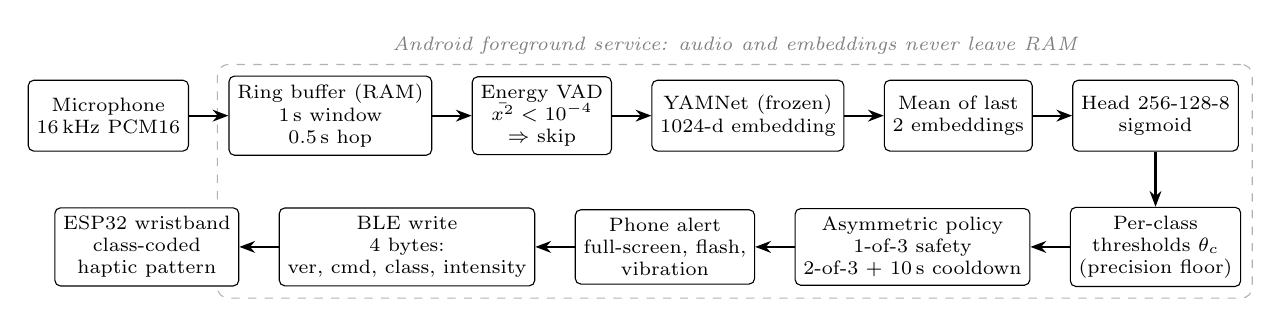
\begin{tikzpicture}[
  node distance=4mm and 5mm,
  box/.style={draw, rounded corners=2pt, align=center, font=\scriptsize, minimum height=9mm, inner sep=3pt, fill=white},
  arr/.style={-{Stealth[length=2mm]}, thick},
  grp/.style={draw=gray!60, dashed, rounded corners=4pt, inner sep=4pt}]
\node[box] (mic) {Microphone\\16\,kHz PCM16};
\node[box, right=of mic] (ring) {Ring buffer (RAM)\\1\,s window\\0.5\,s hop};
\node[box, right=of ring] (vad) {Energy VAD\\$\bar{x^2} < 10^{-4}$\\$\Rightarrow$ skip};
\node[box, right=of vad] (yam) {YAMNet (frozen)\\1024-d embedding};
\node[box, right=of yam] (pool) {Mean of last\\2 embeddings};
\node[box, right=of pool] (head) {Head 256-128-8\\sigmoid};
\node[box, below=7mm of head] (thr) {Per-class\\thresholds $\theta_c$\\(precision floor)};
\node[box, left=of thr] (pol) {Asymmetric policy\\1-of-3 safety\\2-of-3 + 10\,s cooldown};
\node[box, left=of pol] (alert) {Phone alert\\full-screen, flash,\\vibration};
\node[box, left=of alert] (ble) {BLE write\\4 bytes:\\ver, cmd, class, intensity};
\node[box, left=of ble] (band) {ESP32 wristband\\class-coded\\haptic pattern};
\draw[arr] (mic) -- (ring); \draw[arr] (ring) -- (vad); \draw[arr] (vad) -- (yam);
\draw[arr] (yam) -- (pool); \draw[arr] (pool) -- (head); \draw[arr] (head) -- (thr);
\draw[arr] (thr) -- (pol); \draw[arr] (pol) -- (alert); \draw[arr] (alert) -- (ble); \draw[arr] (ble) -- (band);
\begin{scope}[on background layer]
\node[grp, fit=(ring)(vad)(yam)(pool)(head)(thr)(pol)(alert), label={[font=\scriptsize\itshape, gray]above:Android foreground service: audio and embeddings never leave RAM}] {};
\end{scope}
\end{tikzpicture}
\caption{SAHARA pipeline. Everything inside the dashed box runs on the phone. Only a class identifier and an intensity byte cross the BLE link to the wristband.}
\label{fig:arch}
\end{figure*}

Fig.~\ref{fig:arch} shows the pipeline. A native Kotlin foreground service captures 16\,kHz mono audio, so detection continues with the screen off. Samples go into a fixed 1\,s ring buffer that advances every 0.5\,s. A mean-square energy gate ($10^{-4}$) skips silent windows to save power. Each remaining window (the 0.975\,s YAMNet patch) is embedded by a frozen YAMNet into a 1024-dimensional vector. The mean of the two most recent embeddings feeds a classifier head (Dense 256, ReLU, dropout 0.3; Dense 128, ReLU, dropout 0.3; Dense 8, sigmoid) that outputs independent scores for eight classes: smoke alarm, doorbell, siren, knocking, dog bark, baby cry, glass break and appliance beep. The head has $1024{\cdot}256{+}256{+}256{\cdot}128{+}128{+}128{\cdot}8{+}8 = 296{,}328$ parameters, about 1.2\,MB in 32-bit floats. A Flutter user interface shows a flashing full-screen alert, keeps a detection history, and lets the user disable classes and adjust a global sensitivity $s\in[-1,1]$ that scales every threshold as $\theta_c' = \mathrm{clip}(\theta_c(1-0.4s), 0.05, 0.95)$.

\textbf{Privacy.} Audio exists only as floats in the ring buffer and is overwritten every 0.5\,s. Nothing is written to storage, the release manifest has no \texttt{INTERNET} permission, and neither audio, embeddings nor scores cross the BLE link. This differs from ``record and upload'' designs: the system is continuously aware, yet it retains nothing.

% ===========================================================================
\section{Safety-Asymmetric Detection}\label{sec:asym}
% ===========================================================================
We partition the classes into a safety-critical set $\mathcal{S}=\{$smoke alarm, siren, glass break$\}$ and the remaining notification classes $\mathcal{N}$. Asymmetry enters at four points.

\subsection{Cost-weighted training}
The head is trained with a positive-weighted binary cross-entropy
\begin{equation}
\mathcal{L} = -\frac{1}{C}\sum_{c=1}^{C}\Big[w_c\,y_c\log\hat{y}_c + (1-y_c)\log(1-\hat{y}_c)\Big],
\end{equation}
with $w_c=3.0$ for $c\in\mathcal{S}$, $1.5$ for baby cry and appliance beep, and $1.0$ otherwise. A missed positive therefore costs up to three times as much as a false positive, following the standard cost-sensitive formulation~\cite{elkan2001}.

\subsection{Precision-floored threshold calibration}
A single 0.5 threshold is arbitrary for sigmoid outputs trained on imbalanced data. On the validation split we search $\theta\in\{0.10,0.15,\dots,0.90\}$ per class:
\begin{equation}
\theta_c^\ast=\begin{cases}
\arg\max_{\theta} R_c(\theta)\ \text{s.t.}\ P_c(\theta)\ge\pi, & c\in\mathcal{S},\\
\arg\max_{\theta} F_{1,c}(\theta), & c\in\mathcal{N},
\end{cases}
\end{equation}
with precision floor $\pi=0.70$. For a safety class, the system should catch as many true events as possible, but not so many false ones that users learn to ignore it, which is the trust failure reported in~\cite{jain2020homesound}. If no threshold meets the floor, the most precise one is taken and the class is flagged as under-calibrated instead of being reported as fitted.

\subsection{Asymmetric temporal decision rule}\label{sec:policy}
Per-window scores are noisy. A class $c$ fires at step $t$ when its current window is a hit ($s_{c,t}\ge\theta_c$), at least $k_c$ of its last $n=3$ windows are hits, and it has not fired within a 10\,s cooldown. We use $k_c=1$ for $c\in\mathcal{S}$ and $k_c=2$ otherwise.

\textbf{False alarms.} If each background window is a false hit independently with probability $p$, the per-step false-alarm probability is
\begin{equation}
F_k(p)=p\sum_{j=k-1}^{n-1}\binom{n-1}{j}p^{j}(1-p)^{n-1-j},
\end{equation}
so $F_1=p$ and $F_2=p\,(1-(1-p)^2)\approx 2p^2$. At $p=0.05$ the 2-of-3 rule reduces false alarms from 0.05 to 0.0049, a tenfold reduction, and the cooldown further caps alerts at six per minute per class (Fig.~\ref{fig:kofn}). Real windows overlap by 50\,\%, so their errors are positively correlated and the true reduction is smaller; Table~\ref{tab:ablation} measures it empirically.

\textbf{Latency.} Let $W=1$\,s be the window, $H=0.5$\,s the hop and $m=2$ the number of pooled embeddings. Assume that windows lying entirely inside a sustained event score above threshold. The first such window ends at most $W+H$ after onset. The pooled vector is then free of pre-onset audio after $(m-1)$ more hops, and the rule needs $k_c-1$ further hits. The worst-case decision latency is therefore
\begin{equation}
L_c \le W + mH + (k_c-1)H + \tau,
\end{equation}
where $\tau$ is the per-window inference time: $2.0\,\text{s}+\tau$ for safety-critical classes and $2.5\,\text{s}+\tau$ otherwise. Smoothing thus adds no delay to safety classes. In practice, partial windows often clear the threshold earlier.

\begin{figure}[t]
\centering
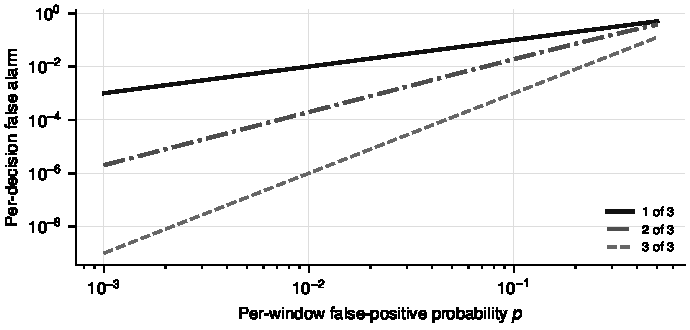
\includegraphics[width=\columnwidth]{figures/kofn.pdf}
\caption{Analytical per-step false-alarm probability of the decision rule as a function of the per-window false-positive rate $p$, assuming independent windows. The 2-of-3 rule used for notification classes reduces false alarms by roughly $2p$ relative to the 1-of-3 rule reserved for safety-critical classes.}
\label{fig:kofn}
\end{figure}

\subsection{Class-coded haptics}
Each alert is sent to the wristband as \texttt{[0x01, 0x01, class, intensity]}. Safety-critical classes always use full intensity (255); for the others the intensity is the confidence scaled to $[128,255]$. The firmware maps each class to a distinct rhythm, so the user can identify the event without looking: smoke alarm uses the ``temporal-three'' pattern of three long pulses that standard fire alarms use~\cite{iso8201}, a siren is a rising and falling swell, a doorbell is a strong then soft ``ding-dong'', and knocking is four quick taps. A new alert interrupts the current one, and dismissing it on the phone sends a STOP command.

% ===========================================================================
\section{Wristband Hardware}\label{sec:band}
% ===========================================================================
The wristband is an ESP32-WROOM-32 BLE peripheral with a 10\,mm coin vibration motor driven through a logic-level MOSFET with 20\,kHz PWM, a 500\,mAh LiPo cell, a protected TP4056 charger and a low-dropout 3.3\,V regulator. Its bill of materials totals about \INR870 at 2026 Indian retail prices (Table~\ref{tab:bom}). To save power the firmware clocks the CPU at 80\,MHz, transmits at $+3$\,dBm, and requests a 30--50\,ms connection interval with slave latency 2, which targets an alert delivery delay below about 150\,ms. When disconnected it advertises every 100\,ms for 30\,s and every 1\,s afterwards. Below 20\,\% charge it lowers motor strength and transmit power, and at 3.4\,V it enters deep sleep. When the phone disconnects, two long buzzes tell the user that alerts have stopped, so a silent wristband never looks the same as a quiet room.

\begin{table}[t]
\caption{Wristband bill of materials (approximate Indian retail prices, 2026)}
\label{tab:bom}
\centering\footnotesize
\begin{tabular}{@{}lr@{}}
\toprule
Component & \INR \\
\midrule
ESP32 DevKit V1 (WROOM-32) & 350 \\
3.7\,V LiPo, 500\,mAh & 180 \\
TP4056 USB-C charger with protection & 35 \\
3.3\,V LDO regulator & 20 \\
10\,mm coin vibration motor & 40 \\
AO3400 MOSFET, diodes, resistors, LED, switch & 31 \\
Perfboard, wiring, headers & 60 \\
Strap and enclosure & 150 \\
\midrule
\textbf{Total} & \textbf{$\approx$870} \\
\bottomrule
\end{tabular}
\end{table}

% ===========================================================================
\section{Data and Evaluation Protocol}\label{sec:data}
% ===========================================================================
\subsection{Public data}
Target clips come from FSD50K~\cite{fonseca2022} (4,494 clips mapped from its ground truth) and AudioSet~\cite{gemmeke2017} (161 downloaded clips, 20--21 per class); background clips come from DESED real soundscapes~\cite{turpault2019} (905 clips). FSD50K has no smoke-alarm or baby-cry label, so these two classes have only 20 AudioSet clips each, and the label distribution is highly skewed (appliance beep 2,093 clips, smoke alarm 20; Table~\ref{tab:data}). Splits are 70/15/15, stratified by class and grouped by recording identifier so that segments of one recording never cross splits.

\subsection{Synthetic Indian-noise mixtures}
To model Indian acoustic conditions at scale, each training target clip is mixed with three random 5\,s chunks of iNoise~\cite{inoise}, which covers autorickshaws, buses, railway stations, streets, homes and workplaces, or of DESED, at an SNR drawn uniformly from $[-5, 10]$\,dB. Mixtures are tagged \texttt{synthetic\_mixed} in every manifest so that real and synthetic results are never conflated.

\subsection{SAHARA-IN field recordings}
Four team members recorded 123 clips (14.6\,min) on their own smartphones. There are 63 target-class clips (16 appliance beep, 16 doorbell, 14 knocking, 11 dog bark, 6 baby cry) and 60 background clips. Backgrounds include street hawkers, a temple, a domestic kitchen, television, monsoon rain, and hard negatives such as drawers, doors and a washing-machine drum spinning without beeping. Across all 123 clips, recording locations are apartments (81), kitchens (11), temples (11), street markets (10) and outdoor rain (10). We split by recorder: clips from two recorders (66) are used for training and those from the other two (57: 34 target, 23 background) are held out, so the test set measures generalisation to unseen people, phones and homes. A separate set of 57 name-call clips (38 positive, 19 negative) of a user's name supports the planned personalisation module (Section~\ref{sec:limits}).

\begin{table}[t]
\caption{Clips per class and source (public data from the committed manifests; SAHARA-IN from the field-recording metadata)}
\label{tab:data}
\centering\footnotesize
\setlength{\tabcolsep}{4pt}
\begin{tabular}{@{}lrrrr@{}}
\toprule
Class & FSD50K & AudioSet & SAHARA-IN & Total \\
\midrule
smoke alarm$^\dagger$ & 0 & 20 & 0 & 20 \\
doorbell & 144 & 20 & 16 & 180 \\
siren$^\dagger$ & 132 & 20 & 0 & 152 \\
knocking & 373 & 29 & 14 & 416 \\
dog bark & 536 & 20 & 11 & 567 \\
baby cry & 0 & 20 & 6 & 26 \\
glass break$^\dagger$ & 1,241 & 34 & 0 & 1,275 \\
appliance beep & 2,068 & 25 & 16 & 2,109 \\
background & DESED 905 & -- & 60 & 965 \\
\bottomrule
\multicolumn{5}{@{}l}{\scriptsize $^\dagger$safety-critical class $\mathcal{S}$.}
\end{tabular}
\end{table}

\subsection{Metrics}
We report per-class average precision (AP) and its macro mean (mAP), as well as precision, recall and F1 at both the default 0.5 and the calibrated thresholds. For streaming behaviour we report false alarms per hour (FA/h) on continuous background audio (DESED, iNoise and SAHARA-IN backgrounds), and we measure latency and energy on a phone. Model selection and calibration use only the validation split.

% ===========================================================================
\section{Results}
% ===========================================================================
\subsection{Baseline on public data}
Table~\ref{tab:baseline} and Fig.~\ref{fig:ap} report the first full baseline, trained on 3,259 clip-level embeddings and tested on 698 held-out clips from FSD50K and AudioSet, without augmentation. Early stopping ended training after 9 epochs, with final validation accuracy 0.810. The model reaches 0.651 mAP. Classes with hundreds of FSD50K clips perform well (dog bark 0.956, glass break 0.937 and appliance beep 0.923 AP). The two AudioSet-only classes fail at the default threshold: smoke alarm reaches only 0.090 AP, and baby cry has zero recall at 0.5 despite 0.669 AP. Each has three test clips, so their per-class estimates carry wide uncertainty. Siren, a safety-critical class with 152 clips, reaches only 0.250 AP. Two lessons follow. For safety-critical classes, the bottleneck is data, not model capacity. And mAP alone hides failures that matter most to the user, which motivates per-class, safety-weighted reporting.

\begin{table}[t]
\caption{Baseline test results (698 clips, threshold 0.5)}
\label{tab:baseline}
\centering\footnotesize
\begin{tabular}{@{}lrrrr@{}}
\toprule
Class & Precision & Recall & F1 & AP \\
\midrule
smoke alarm$^\dagger$ & 0.000 & 0.000 & 0.000 & 0.090 \\
doorbell & 0.682 & 0.395 & 0.500 & 0.632 \\
siren$^\dagger$ & 0.333 & 0.333 & 0.333 & 0.250 \\
knocking & 0.826 & 0.655 & 0.731 & 0.751 \\
dog bark & 1.000 & 0.893 & 0.943 & 0.956 \\
baby cry & 0.000 & 0.000 & 0.000 & 0.669 \\
glass break$^\dagger$ & 0.881 & 0.895 & 0.888 & 0.937 \\
appliance beep & 0.860 & 0.790 & 0.824 & 0.923 \\
\midrule
\textbf{Macro} & \textbf{0.573} & \textbf{0.495} & \textbf{0.527} & \textbf{0.651} \\
\bottomrule
\end{tabular}
\end{table}

\begin{figure}[t]
\centering
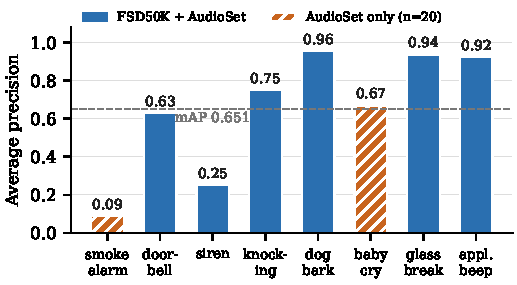
\includegraphics[width=\columnwidth]{figures/baseline_ap.pdf}
\caption{Per-class test AP of the baseline. The hatched classes have only 20 public clips each (AudioSet), and three test clips each.}
\label{fig:ap}
\end{figure}

\subsection{Effect of threshold calibration}
Table~\ref{tab:calib} shows the calibrated thresholds on the validation split. Calibration lowers most thresholds well below 0.5 and raises recall: knocking from 0.390 to 0.576, doorbell from 0.304 to 0.500, and baby cry from 0.667 to 1.000 at unchanged precision. Glass break trades precision (0.830 to 0.714) for recall (0.852 to 0.926) while keeping precision above the 0.70 floor, which is exactly what the constraint is designed to do. For smoke alarm, no threshold met the floor (best precision 0.25), so the calibrator flags the class as under-calibrated instead of hiding the problem. These are validation-set figures; the corresponding test-set results are in Table~\ref{tab:full}.

\begin{table}[t]
\caption{Per-class threshold calibration on the validation split (default 0.5 $\rightarrow$ calibrated $\theta^\ast$)}
\label{tab:calib}
\centering\footnotesize
\setlength{\tabcolsep}{3.5pt}
\begin{tabular}{@{}lrrrrr@{}}
\toprule
Class & $\theta^\ast$ & P@0.5 & P@$\theta^\ast$ & R@0.5 & R@$\theta^\ast$ \\
\midrule
smoke alarm$^\dagger$ & 0.15 & 0.000 & 0.250 & 0.000 & 0.333 \\
doorbell & 0.20 & 0.583 & 0.426 & 0.304 & 0.500 \\
siren$^\dagger$ & 0.40 & 1.000 & 1.000 & 0.333 & 0.333 \\
knocking & 0.15 & 0.719 & 0.680 & 0.390 & 0.576 \\
dog bark & 0.30 & 0.972 & 0.960 & 0.854 & 0.878 \\
baby cry & 0.10 & 1.000 & 1.000 & 0.667 & 1.000 \\
glass break$^\dagger$ & 0.25 & 0.830 & 0.714 & 0.852 & 0.926 \\
appliance beep & 0.50 & 0.858 & 0.858 & 0.847 & 0.847 \\
\bottomrule
\end{tabular}
\end{table}

\subsection{Full model and generalisation to Indian conditions}
Table~\ref{tab:full} reports the final model, trained at window level (1\,s, matching on-device inference) on public data, synthetic Indian-noise mixtures and the SAHARA-IN training recorders. It is evaluated on three test sets of increasing difficulty: the public held-out split, synthetic mixtures at fixed SNRs, and the recorder-disjoint SAHARA-IN split.

\begin{table}[t]
\caption{Final model on three test sets (calibrated thresholds)}
\label{tab:full}
\centering\footnotesize
\setlength{\tabcolsep}{3.5pt}
\begin{tabular}{@{}lrrrr@{}}
\toprule
Test set & mAP & Macro R & Safety R & FA/h \\
\midrule
Public held-out split & \tbd & \tbd & \tbd & -- \\
Synthetic mix, SNR 10\,dB & \tbd & \tbd & \tbd & -- \\
Synthetic mix, SNR 0\,dB & \tbd & \tbd & \tbd & -- \\
Synthetic mix, SNR $-5$\,dB & \tbd & \tbd & \tbd & -- \\
SAHARA-IN (unseen recorders) & \tbd & \tbd & -- & \tbd \\
Background stream (DESED, iNoise) & -- & -- & -- & \tbd \\
\bottomrule
\end{tabular}
\end{table}

\TBD{2--3 sentences interpreting Table~\ref{tab:full}: the drop from public to SAHARA-IN, which classes transfer, and FA/h against a target of fewer than one alert per hour.}

\subsection{Ablation of the asymmetric components}
Table~\ref{tab:ablation} isolates each safety-asymmetric component, measured on the public test split (safety-class recall) and on continuous background audio (FA/h).

\begin{table}[t]
\caption{Ablation (public test split; FA/h on continuous background)}
\label{tab:ablation}
\centering\footnotesize
\setlength{\tabcolsep}{3.5pt}
\begin{tabular}{@{}lrrr@{}}
\toprule
Configuration & mAP & Safety R & FA/h \\
\midrule
Unweighted BCE, $\theta=0.5$, 1-of-1 & \tbd & \tbd & \tbd \\
+ cost-weighted BCE & \tbd & \tbd & \tbd \\
+ precision-floored calibration & \tbd & \tbd & \tbd \\
+ 2-of-3 for all classes & \tbd & \tbd & \tbd \\
+ asymmetric 1-of-3 / 2-of-3 (SAHARA) & \tbd & \tbd & \tbd \\
\bottomrule
\end{tabular}
\end{table}

\subsection{On-device cost}
Table~\ref{tab:device} reports the deployment cost on \TBD{phone model, Android version}. The classifier head adds 296,328 parameters to YAMNet's roughly 3.7 million~\cite{yamnet}.

\begin{table}[t]
\caption{On-device cost}
\label{tab:device}
\centering\footnotesize
\begin{tabular}{@{}lr@{}}
\toprule
Measure & Value \\
\midrule
Head parameters & 296,328 \\
TFLite size, FP32 / INT8 (YAMNet + head) & \tbd\ / \tbd\ MB \\
INT8 mAP change vs.\ FP32 & \tbd \\
Inference time per window (median / p95) & \tbd\ / \tbd\ ms \\
End-to-end latency, onset to phone alert & \tbd\ s \\
Phone alert to wristband vibration & \tbd\ ms \\
Phone battery drain, service running & \tbd\ \%/h \\
Wristband current, connected idle & \tbd\ mA \\
Wristband life, 500\,mAh & \tbd\ h \\
\bottomrule
\end{tabular}
\end{table}

% ===========================================================================
\section{Discussion and Limitations}\label{sec:limits}
% ===========================================================================
\textbf{Data scarcity for the most critical classes.} The baseline shows that smoke alarm and baby cry, which have the highest stakes, have the least public data. SAHARA-IN does not yet contain smoke-alarm, siren or glass-break recordings because they are hard to record safely. Targeted collection (for example, a controlled smoke-alarm test with the building's consent) is our most valuable next step.

\textbf{Small field set.} With 123 clips and a recorder split that leaves some classes on only one side, SAHARA-IN measures transfer for doorbell, dog bark and appliance beep, plus false alarms on Indian backgrounds, but it cannot estimate every class. We release the protocol so that the set can grow.

\textbf{Independence assumption.} The false-alarm analysis assumes independent windows. Overlapping windows are correlated, so the analysis is an upper bound on the benefit; Table~\ref{tab:ablation} reports the measured effect.

\textbf{No user study yet.} We have not yet evaluated SAHARA with DHH participants. Prior work shows that perceived usefulness depends on false-alarm rates and on notification design~\cite{jain2020homesound,findlater2019}. A field deployment with DHH users in Mumbai, measuring missed events, alert fatigue and haptic-pattern recognition, is planned.

\textbf{Personalisation.} Users want to be alerted when someone calls their name. We have collected a name-call set, and plan to fuse a few-shot prototypical module~\cite{snell2017,jain2022protosound} with the main head, so that users can enrol their own name and household sounds on the device.

% ===========================================================================
\section{Conclusion}
% ===========================================================================
SAHARA shows that an assistive sound-awareness system can encode the unequal cost of missed safety sounds at every stage, from the loss to the vibration pattern, while running entirely on a phone and a \INR870 wristband and retaining no audio. Our baseline results show that mAP alone hides the failures that matter most, and that the classes users depend on most have the least data. We release the code, the BLE protocol, the firmware and the SAHARA-IN evaluation protocol to support safety-aware, privacy-preserving and regionally representative assistive audio research.

\section*{Acknowledgment}
\TBD{Thank the guide and department; mention any funding.}

\begin{thebibliography}{99}
\bibitem{who2021} World Health Organization, \emph{World Report on Hearing}. Geneva: WHO, 2021.
\bibitem{census2011} Office of the Registrar General \& Census Commissioner, India, ``Census of India 2011: Data on disability,'' 2011.
\bibitem{findlater2019} L.~Findlater, B.~Chinh, D.~Jain, J.~Froehlich, R.~Kushalnagar, and A.~C.~Lin, ``Deaf and hard-of-hearing individuals' preferences for wearable and mobile sound awareness technologies,'' in \emph{Proc. CHI}, 2019.
\bibitem{bragg2016} D.~Bragg, N.~Huynh, and R.~E.~Ladner, ``A personalizable mobile sound detector app design for deaf and hard-of-hearing users,'' in \emph{Proc. ASSETS}, 2016.
\bibitem{gemmeke2017} J.~F.~Gemmeke \emph{et al.}, ``Audio Set: An ontology and human-labeled dataset for audio events,'' in \emph{Proc. IEEE ICASSP}, 2017, pp.~776--780.
\bibitem{laput2018} G.~Laput, K.~Ahuja, M.~Goel, and C.~Harrison, ``Ubicoustics: Plug-and-play acoustic activity recognition,'' in \emph{Proc. UIST}, 2018.
\bibitem{jain2020soundwatch} D.~Jain, H.~Ngo, P.~Patel, S.~Goodman, L.~Findlater, and J.~Froehlich, ``SoundWatch: Exploring smartwatch-based deep learning approaches to support sound awareness for deaf and hard of hearing users,'' in \emph{Proc. ASSETS}, 2020.
\bibitem{jain2020homesound} D.~Jain \emph{et al.}, ``HomeSound: An iterative field deployment of an in-home sound awareness system for deaf or hard of hearing users,'' in \emph{Proc. CHI}, 2020.
\bibitem{jain2022protosound} D.~Jain, K.~H.~A.~Nguyen, S.~Goodman, R.~Grossman-Kahn, H.~Ngo, A.~Kusupati, R.~Du, A.~Olwal, L.~Findlater, and J.~E.~Froehlich, ``ProtoSound: A personalized and scalable sound recognition system for deaf and hard-of-hearing users,'' in \emph{Proc. CHI}, 2022.
\bibitem{iso8201} ISO 8201:2017, \emph{Alarm systems -- Audible emergency evacuation signal -- Requirements}. International Organization for Standardization, 2017.
\bibitem{inoise} S.~K.~Kopparapu, I.~Sheikh, and S.~Thanneeru, ``iNoise: Indian noise database,'' IEEE DataPort, doi: 10.21227/w3xm-jn45.
\bibitem{matthews2006} T.~Matthews, J.~Fong, F.~W.-L.~Ho-Ching, and J.~Mankoff, ``Evaluating non-speech sound visualizations for the deaf,'' \emph{Behaviour \& Information Technology}, vol.~25, no.~4, pp.~333--351, 2006.
\bibitem{snell2017} J.~Snell, K.~Swersky, and R.~Zemel, ``Prototypical networks for few-shot learning,'' in \emph{Proc. NeurIPS}, 2017.
\bibitem{goodman2021} S.~M.~Goodman \emph{et al.}, ``Toward user-driven sound recognizer personalization with people who are d/Deaf or hard of hearing,'' \emph{Proc. ACM IMWUT}, vol.~5, no.~2, 2021.
\bibitem{hershey2017} S.~Hershey \emph{et al.}, ``CNN architectures for large-scale audio classification,'' in \emph{Proc. IEEE ICASSP}, 2017, pp.~131--135.
\bibitem{kong2020} Q.~Kong, Y.~Cao, T.~Iqbal, Y.~Wang, W.~Wang, and M.~D.~Plumbley, ``PANNs: Large-scale pretrained audio neural networks for audio pattern recognition,'' \emph{IEEE/ACM Trans. Audio, Speech, Lang. Process.}, vol.~28, pp.~2880--2894, 2020.
\bibitem{yamnet} M.~Plakal and D.~Ellis, ``YAMNet,'' TensorFlow Model Garden, 2020. [Online]. Available: \url{https://github.com/tensorflow/models/tree/master/research/audioset/yamnet}
\bibitem{howard2017} A.~G.~Howard \emph{et al.}, ``MobileNets: Efficient convolutional neural networks for mobile vision applications,'' arXiv:1704.04861, 2017.
\bibitem{jacob2018} B.~Jacob \emph{et al.}, ``Quantization and training of neural networks for efficient integer-arithmetic-only inference,'' in \emph{Proc. IEEE CVPR}, 2018, pp.~2704--2713.
\bibitem{fonseca2022} E.~Fonseca, X.~Favory, J.~Pons, F.~Font, and X.~Serra, ``FSD50K: An open dataset of human-labeled sound events,'' \emph{IEEE/ACM Trans. Audio, Speech, Lang. Process.}, vol.~30, pp.~829--852, 2022.
\bibitem{turpault2019} N.~Turpault, R.~Serizel, A.~Parag Shah, and J.~Salamon, ``Sound event detection in domestic environments with weakly labeled data and soundscape synthesis,'' in \emph{Proc. DCASE Workshop}, 2019.
\bibitem{mesaros2021} A.~Mesaros, T.~Heittola, T.~Virtanen, and M.~D.~Plumbley, ``Sound event detection: A tutorial,'' \emph{IEEE Signal Process. Mag.}, vol.~38, no.~5, pp.~67--83, 2021.
\bibitem{elkan2001} C.~Elkan, ``The foundations of cost-sensitive learning,'' in \emph{Proc. IJCAI}, 2001, pp.~973--978.
\end{thebibliography}

\end{document}
